\section{Transformada Rápida de Fourier}

\begin{frame}[fragile]{DFT em $O(N\log N)$}

    \begin{itemize}
        \item A divisão e conquista pode ser aplicada no cálculo da DFT para reduzir sua
            complexidade assintótica

        \item Na etapa de divisão o sinal é dividido em duas partes de tamanhos aproximadamente
            iguais

        \item A conquista acontece quando o sinal tem uma única amostra: neste caso a transformada
            discreta coincide com a própria amostra

        \item A fusão permite o cálculo da DFT do sinal a partir das DFTs das duas partes

        \item Se a fusão for feita em $O(N)$, a recorrência se torna
        \[
            f(N) = 2f(N/2) + O(N)
        \]

        \item O Teorema Mestre nos diz que a complexidade da transformada passa a ser $O(N\log N)$

        \item Esta versão da DFT é denominada \textit{Fast Fourier Transform} (FFT)
    \end{itemize}

\end{frame}

\begin{frame}[fragile]{Decomposição do sinal FFT}

    \begin{itemize}
        \item Considere o sinal $(a_k) = a_0, a_1, \ldots, a_{N-1}$

        \item Assuma, sem perda de generalidade, que $N = 2^t$, para algum $t$ natural

        \item Se $N$ não for uma potência de dois, basta adicionar um número suficiente de amostras
            $a_i = 0$ ao sinal até que $N$ se torne uma potência de dois

        \item A etapa de divisão, também denominada decomposição do sinal, o sinal é separado
            em duas partes de tamanho $N/2$: as amostras cujos índices são pares $(e_k)$ e as 
            amostras cujos índices são ímpares $(o_k)$

        \item Assim,
        \[
            (e_k) = a_0, a_2, a_4, \ldots, a_{N - 2}
        \]
        e
        \[
            (o_k) = a_1, a_3, a_5, \ldots, a_{N - 1}
        \]
    \end{itemize}

\end{frame}

\input{divide_view}

\begin{frame}[fragile]{Decomposição $\times$ ordenação}

    \begin{itemize}
        \item Gerando a decomposição por meio da alocação de novos dois subvetores com as cópias
            dos elementos de índices pares e ímpares permite uma implementação \textit{top-down}
            da FFT

        \item Para uma implementação \textit{bottom-up}, é preciso entender
            o padrão subjacente que surge desta decomposição

        \item De fato, os elementos que ocupam as folhas nas árvores de decomposição tem índices
            que correspondem à ordenação dos números $\{ 0, 1, 2, \ldots, N - 1\}$ usando como
            critério a inversão de sua representação binária

        \item Assim, por meio de um comparador customizado este ordenação pode ser feita 
            com complexidade $O(N\log N)$, o que não modifica a complexidade da FFT como um todo
    \end{itemize}

\end{frame}

\input{order_view}

\begin{frame}[fragile]{Implementação da ordenação por padrão binário}
    \inputsnippet{cpp}{1}{17}{codes/order.cpp}
\end{frame}

\begin{frame}[fragile]{Implementação da ordenação por padrão binário}
    \inputsnippet{cpp}{19}{38}{codes/order.cpp}
\end{frame}

\begin{frame}[fragile]{Conquista}

    \begin{itemize}
        \item A etapa de conquista acontece em sinais como uma única amostra

        \item Aplicando o valor $N = 1$ na transformada discreta obtêm-se
        \[
            X_0 = \sum_{n = 0}^{N - 1} x_ne^{-2\pi ikn/N} = 
                \sum_{n = 0}^0 x_ne^{-2\pi kn} = x_0
        \]

        \item Assim, a própria amostra corresponde à sua transformada

        \item É preciso atentar, contudo, que embora numericamente iguais, $X_0$ reside no 
            domínio das frequências, enquanto que $x_0$ está no domínio do tempo

        \item Portanto esta etapa tem complexidade $O(1)$

    \end{itemize}

\end{frame}

\begin{frame}[fragile]{Fusão (Síntese)}

    \begin{itemize}
        \item A última etapa consiste em combinar as transformadas das duas partes (pares e
            ímpares) na transformada do sinal

        \item Lembrando que a Transformada de Fourier é linear, a transformada de um sinal $x_k$
            pode ser computada como a soma de dois sinais distintos cuja soma resulte em $x_k$

        \item Considere os sinais $e_k$ e $o_k$ dados por
        \[
            e_i = \left\{ \begin{array}{ll}
                    x_i, &\mbox{se}\ i\ \mbox{é par}\\
                    0, &\mbox{caso contrário}
                \end{array}\right.
        \]
        e
        \[
            o_j = \left\{ \begin{array}{ll}
                    x_j, &\mbox{se}\ j\ \mbox{é ímpar}\\
                    0, &\mbox{caso contrário}
                \end{array}\right.
        \]
 
    \end{itemize}

\end{frame}

\begin{frame}[fragile]{Fusão (Síntese)}

    \begin{itemize}
        \item Deste modo, $x_k = e_k + o_k$

        \item As transformadas de $e_k$ e $o_k$ tem um comportamento peculiar

        \item A transformada de $e_k$ duplica seus resultados

        \item A transformada de $o_k$ tem mesmo comportamento, porém com os valores multiplicados
            por uma componente sinusoidal

        \item Isto porque, em relação à $x_k$, o sinal $o_k$ está deslocado no tempo em uma
            unidade

        \item Deslocar no tempo corresponde a convolução do sinal com uma função $\delta(t - a)$,
            onde $a$ é o deslocamento

        \item A transformada da função $\delta(t - a)$ é uma exponencial complexa:
        \[
            \mathcal{F}[\delta(t - a)] = \int_{-\infty}^{\infty} \delta(t - a)e^{-2\pi kit}dt =
                e^{-2\pi kai}
        \]
    
    \end{itemize}

\end{frame}

\input{synthesis_view}

\begin{frame}[fragile]{Padrão borboleta}

    \begin{itemize}
        \item Como as transformadas das duas partes foram computadas sem o deslocamento, é preciso
            compensá-lo na composição da transformada do todo

        \item As componentes oriundas da parte par $E_k$ são somadas sem alteração em cada
            componente da transformada $X_k$

        \item Já as componentes de $O_k$ devem ser multiplicadas pela componente 
        \[
            s_k = e^{\frac{2\pi ki}{N}}
        \]
        antes de serem somadas

        \item Esta multiplicação afeta o sinal do termo: a primeira metade terá sinal negativo e
            a segunda metade sinal positivo

        \item Este ajuste é denominado padrão borboleta, por conta da visualização do diagrama
            gerado
    \end{itemize}

\end{frame}

\begin{frame}[fragile]{Padrão borboleta para $N = 2$}

    \begin{figure}
        \centering

        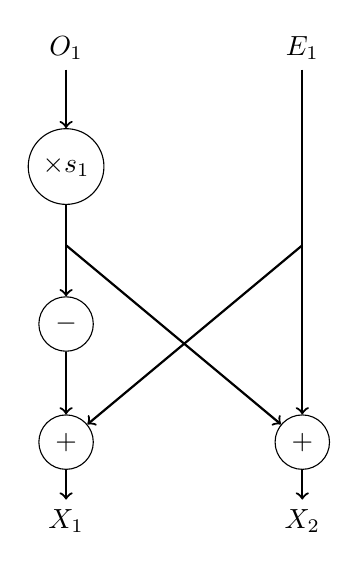
\begin{tikzpicture}
            \node (A) at (0, 5) { $O_1$ };
            \node[draw,circle] (B) at (0, 3.5) { $\times s_1$ };
            \node[draw,circle] (C) at (0, 1.5) { $\mathbf{-}$ };
            \node[draw,circle] (D) at (0, 0) { $\mathbf{+}$ };
            \node (E) at (0, -1) { $X_1$ };

            \node (F) at (3, 5) { $E_1$ };
            \node[draw,circle] (G) at (3, 0) { $\mathbf{+}$ };
            \node (H) at (3, -1) { $X_2$ };
            \coordinate (I) at (3, 2.5);
            \coordinate (J) at (0, 2.5);

            \draw[thick,->] (A) edge (B);
            \draw[thick,->] (B) edge (C);
            \draw[thick,->] (C) edge (D);
            \draw[thick,->] (D) edge (E);

            \draw[thick,->] (F) edge (G);
            \draw[thick,->] (G) edge (H);
            \draw[thick,->] (I) -- (D);
            \draw[thick,->] (J) -- (G);


        \end{tikzpicture}

    \end{figure}

\end{frame}


